% AmphionTS-Bench. Sources: refs/docs/ts_benchmark.md §1--4; HTML §2 (tables 1--2).
% Counts verified against the AmphionEval records of the v12 benchmark
% (248 subsets, 12,950 present / 11,151 absent).

\section{\tsbench: A TS-ASR Benchmark for Real-World Conditions}
\label{sec:benchmark}

\tsbench aims to make evaluation scores agree with behavior in real use.
It is a Mandarin benchmark with a synthetic part and a real part, and it will be released publicly.
\Cref{tab:bench_vs_common} contrasts it with common evaluations, and \Cref{fig:bench} shows how its samples are built.

\begin{figure}[t]
  \centering
  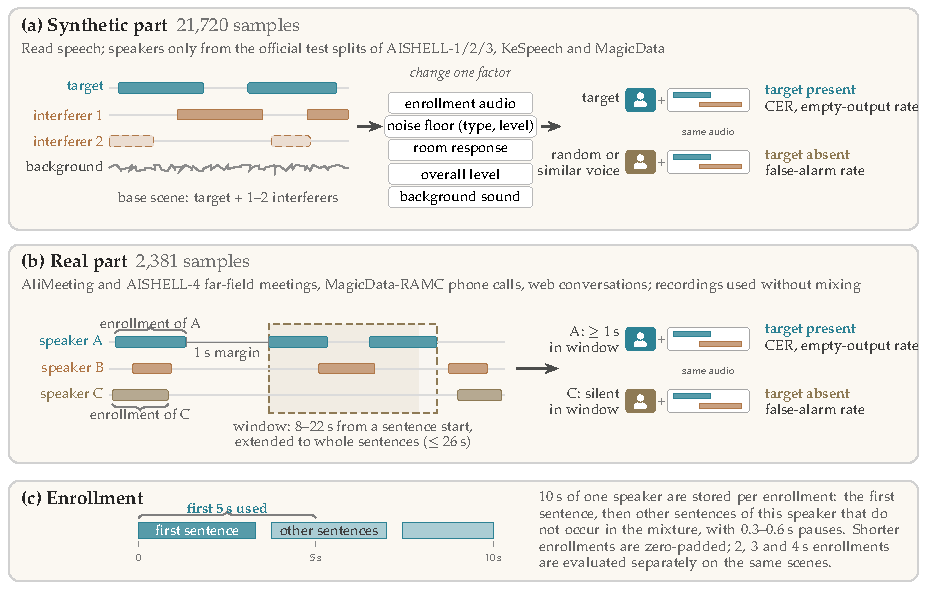
\includegraphics[width=\linewidth]{figures/bench-construction.pdf}
  \caption{Construction of \tsbench. (a)~Synthetic part: on base scenes of the target and one or two interferers (dashed: the second interferer), one factor is changed at a time. (b)~Real part: recordings are cut into windows without mixing, and the enrollment comes from the same recording outside the window. In both parts, every mixture yields a target-present and a target-absent sample with identical audio that differ only in the enrollment; for the absent sample it belongs to a random person or to one of the five speakers closest to an interferer (synthetic), or to a speaker of the same recording who is silent in the window (real). (c)~Each enrollment stores 10\,s of one speaker, and the first 5\,s are used.}
  \label{fig:bench}
\end{figure}

\begin{table}[t]
  \caption{\tsbench compared with common TSE and TS-ASR evaluations.}
  \label{tab:bench_vs_common}
  \centering
  \small
  \begin{tabularx}{\linewidth}{@{}l>{\raggedright\arraybackslash}p{3.6cm}>{\raggedright\arraybackslash}X@{}}
    \toprule
     & Common evaluations & \tsbench \\
    \midrule
    Speech & Synthetic mixtures of read speech & Synthetic mixtures of read speech; real meeting, phone-call and web-conversation recordings, not mixed \\
    Talkers & 2--3 & 0--5 in the synthetic part; real windows split into 1, 2 and 3+ talkers \\
    Target presence & Always present & Every condition has present and absent groups; 11{,}151 absent samples \\
    Timing & Utterances overlaid with random delays & Continuous speech, interjections, mid-clip entry or exit, turn-taking, simultaneous starts, hand-overs, about 1\,s of speech \\
    Enrollment & Another clean utterance of the same person & First 5\,s; only 2--4\,s recorded, only 1\,s of speech, leading silence, narrowband, noise, reverberation, another voice mixed in, very quiet; enrollments from real meetings \\
    Acoustics & Clean, or with synthetic noise and reverberation & Real ambient noise floors, measured and simulated room responses, near-field and far-field mismatch, level and recording chain, babble and environmental events \\
    Nobody speaking & Usually absent & Noise, music, traffic, near silence, babble, crowds, songs with vocals \\
    Metrics & SDR or WER with the target present & Target-present CER and empty-output rate, target-absent false-alarm rate \\
    \bottomrule
  \end{tabularx}
  \par\smallskip
  {\footnotesize Common evaluations are test sets synthesized from read speech, such as WSJ0-2mix~\cite{hershey2016deep}, Libri2Mix~\cite{cosentino2020librimix}, WHAM!~\cite{wichern2019wham}, WHAMR!~\cite{maciejewski2020whamr} and LibriSpeechMix~\cite{kanda2020serialized}; their exact settings vary.\par}
\end{table}

\subsection{Design principles}
\label{subsec:bench_principles}

\paragraph{Both kinds of error are scored.}
Every condition has a target-present and a target-absent group, and the 11{,}151 absent samples make up nearly half of the benchmark.
Present samples report CER and the empty-output rate, and absent samples report the false-alarm rate.
The three metrics must be read together: a model that merely suppresses false alarms also drops the enrolled speaker's speech, which appears as a higher empty-output rate.

\paragraph{Scenes come from errors observed in real use.}
Each subset corresponds to a specific failure hypothesis rather than a random combination of conditions.
During continuous listening, for example, voice activity detection may cut a 1.2--6\,s segment in which only someone else speaks.
Other examples are the enrolled speaker finishing a sentence and another person replying with a sentence that starts the same way, a similar-sounding person saying one short phrase of 0.5--1.6\,s, only a song with vocals playing, and a user who spoke for only 2--4\,s when enrolling.

\paragraph{Paired, single-factor conditions.}
The synthetic part draws scenes, enrollments and backgrounds from three independent random streams.
Each base scene has the target and one or two interferers.
On these scenes, a single factor is changed at a time: the enrollment audio, the type and level of the noise floor, the room response, the overall level or the background sound.
Absent samples are paired as well: the mixture is identical item by item, and only the enrollment changes.
The new enrollment belongs to a random person or to one of the five speakers whose embeddings are closest to an interferer in the mixture.
Differences between such conditions are therefore paired differences in that one factor.

\paragraph{Real recordings without mixing.}
The real part comes from the human-annotated test sets of the AliMeeting~\cite{yu2022m2met} and AISHELL-4~\cite{fu2021aishell4} far-field meetings (first array channel) and the MagicData-RAMC~\cite{yang2022open} phone calls, plus multi-party web conversations from Emilia~\cite{he2024emilia} with pseudo-labels.
A window starts at the beginning of a sentence, spans 8--22\,s, and is extended to include every complete sentence that overlaps it, up to 26\,s; windows do not overlap.
Each window yields a target-present sample, for someone who speaks for at least 1\,s in it, and a target-absent sample with identical audio.
The absent sample enrolls someone from the same recording who does not speak in the window or, if there is no such person, a speaker from another recording of the same corpus.
The enrollment is taken from the same recording outside the window, with a 1\,s margin.
The same AliMeeting windows also come in four combinations of near-field (headset) and far-field audio for the enrollment and the mixture, which we use to calibrate the synthetic far-field conditions (\Cref{subsec:exp_conditions}).

\paragraph{An enrollment protocol matched to deployment.}
Each enrollment stores 10\,s of the same speaker: the first sentence is followed by other sentences of this person that do not occur in the mixture, with 0.3--0.6\,s pauses between them.
As in deployment, the first 5\,s are used at evaluation time, and shorter enrollments are zero-padded.
Enrollments of only 2, 3 or 4\,s are evaluated separately on the same scenes.

\paragraph{Speaker splits and label checks.}
Synthetic speakers come only from the official test splits of AISHELL-1~\cite{bu2017aishell1}, AISHELL-2~\cite{du2018aishell2}, AISHELL-3~\cite{shi2021aishell3}, KeSpeech~\cite{tang2021kespeech} and MagicData.
In the real windows, presence and absence follow the human-annotated utterance timeline.
Samples whose first 5\,s of enrollment contain at least 0.3\,s of another speaker are reported separately as ``enrollment contains another voice'' and are not scored as clean enrollments.
We also checked with speaker embeddings that each enrollment really belongs to the target, replaced three AISHELL-4 enrollments that belonged to another participant, and removed one window whose target could not be confirmed.

\subsection{Composition}
\label{subsec:bench_composition}

\Cref{tab:bench_composition} lists the size of each section.
The synthetic part has 21{,}720 samples and the real part 2{,}381; each synthetic subset has 120 or 150 samples, and the real subsets are split by corpus and by the number of speakers in the window.
Twelve diagnostic subsets count toward the overall results but not toward any section.
\Cref{app:synthesis} gives the mixing rules of the synthetic part.

\begin{table}[t]
  \caption{Composition of \tsbench (number of samples).}
  \label{tab:bench_composition}
  \centering
  \small
  \begin{tabularx}{\linewidth}{@{}>{\raggedright\arraybackslash}p{3.0cm}>{\raggedright\arraybackslash}Xrrr@{}}
    \toprule
    Section & Content & Subsets & Present & Absent \\
    \midrule
    Degraded enrollment & Only the enrollment changes on the same base scenes: 1\,s of speech, leading silence, 4\,kHz narrowband, noise, reverberation, another voice, very quiet, only 2--4\,s recorded & 22 & 1{,}650 & 1{,}650 \\
    Entry, exit and number of interferers & Target speaks throughout, interjects, enters or leaves mid-clip, takes turns, starts together with someone, says about 1\,s, is quieter than others; 1--4 interferers; absent cases with similar voices and with long and short clips; hand-overs & 27 & 2{,}280 & 960 \\
    Short segments & 1.2--6\,s voice-activity segments with only others speaking; another person says one 0.5--1.6\,s phrase; the enrolled speaker alone says a short phrase, plus quiet, far-field and noisy variants & 15 & 2{,}520 & 1{,}080 \\
    No one speaking & Noise, music, traffic, near silence, babble, crowds, environmental events, songs with vocals & 10 & 0 & 1{,}200 \\
    Environmental noise and recording chain & Reverberation with noise, background music, traffic, phone and studio recordings; noise-floor type and level; overall level; babble, crowds and environmental events & 52 & 3{,}240 & 3{,}000 \\
    Far field and room reverberation & Measured and simulated rooms; room responses on the target, the interferers or both; near-field and far-field mismatch between enrollment and mixture & 22 & 1{,}320 & 1{,}320 \\
    Real meetings, phone calls and web conversations & AliMeeting and AISHELL-4 far-field meetings, MagicData-RAMC phone calls, web conversations; split by talkers per window; four AliMeeting near/far combinations; enrollments containing another voice reported separately & 88 & 1{,}190 & 1{,}191 \\
    Diagnostic conditions & 0\,dB enrollment contamination, clipping, 3.4\,kHz narrowband, $\mu$-law coding, stacked outdoor and office conditions & 12 & 750 & 750 \\
    \midrule
    Total & & 248 & 12{,}950 & 11{,}151 \\
    \bottomrule
  \end{tabularx}
  \par\smallskip
  {\footnotesize Synthetic speakers come only from the official test splits of their corpora; the real part comes only from test sets and web conversations. Diagnostic subsets count toward the overall results but not toward any section; a subset that matches two sections is counted once, in the first.\par}
\end{table}

\subsection{Metrics}
\label{subsec:bench_metrics}

Mandarin, including dialects, is scored by character.
Before scoring, text is converted to simplified characters, numbers are normalized, and filler words such as \emph{e} and \emph{a} (in pinyin) are removed.
CER is pooled as the total number of character errors over all target-present samples divided by the total number of reference characters.
The \emph{empty-output rate} is the share of target-present samples whose normalized output is empty (a whole-utterance miss), and the \emph{false-alarm rate} is the share of target-absent samples whose normalized output is not empty.
Overall results are pooled over all subsets, and section results over the subsets of that section.
When the same model was run twice during development, the false-alarm rate of a single subset differed by 0.4 points on average and by at most 1.7 points, and its CER by 0.5 points on average and by at most 1.9 points.
Smaller differences on a single subset should not be over-read.
